\appendix

\chapter{A Chemical Plant Example}\label{app:alarm}

This appendix presents the requirements for a simple alarm system for a
chemical plant. It forms a running example that serves to illustrate
the process described earlier and to introduce elements of the VDM++
modelling language. Although the modelling process is described here
as though it were a single-pass activity, a real development would
usually be iterative. 


\section{An informal description}

The example is inspired by a subcomponent of a large
alarm system developed by IFAD A/S and introduced in 
\cite{Fitzgerald&98b}.  A model of the
system will be developed and validated using the facilities of
Enterprise Architect and Overture
%Rational 
%Rose$^{\mbox{\small\textbf{{\textregistered}}}}$\ and 
%\vdmtools$^{\mbox{\small\textbf{{\textregistered}}}}$, 
%including the Rose-VDM++ Link, 
enabling a graphical overview
of the model in the form of UML class diagrams and sequence diagrams
corresponding to traces.
Chapter~\ref{cha:toolbox} provides an interactive and hands-on tour of
the tools available for supporting the development of the model.

Imagine that you are developing a system that manages the calling out
of experts to deal with operational faults discovered in a chemical
plant.  The plant is equipped with sensors that are able to raise
alarms in response to conditions in the plant.  When an alarm is
raised, an expert must be called to the scene.  Experts have different
qualifications for coping with different kinds of alarms. It has been
decided to produce a model to ensure that the rules
concerning the duty schedule and the calling out of experts are
correctly understood and implemented. The individual requirements are
labelled R1, R8 for further reference:

\begin{reqs}
\item A computer-based system is to be developed to manage the alarms 
of this plant.
\item Four kinds of qualifications are needed to cope with the alarms: 
 electrical, mechanical, biological, and chemical.
\item There must be experts on duty during all periods allocated in 
the system.
\item Each expert can have a list of qualifications.
\item Each alarm reported to the system has a qualification associated 
with it along with a description of the alarm that can be understood 
by the expert.
\item Whenever an alarm is received by the system an expert with the 
right qualification should be found so that he or she can be 
paged.
\item The experts should be able to use the system database to check 
when they will be on duty.
\item It must be possible to assess the number of experts on duty.
\end{reqs}

In the next section the development of a model of an alarm
system to meet these requirements is initiated. The purpose of the model is to
clarify the rules governing the duty roster and calling out of experts
to deal with alarms.

\section{A VDM++ model of the Alarm example}\label{sec:VDMModel}

This section presents the UML class diagram and the full VDM++ model
of the alarm example. However, it does so without any explanatory
text. That is placed in the VDM++ book so if you are a newcommer to
VDM++ please read that there.

\subsection{A UML Class Diagram}

In Figure~\ref{fig:finalumlforalarm} the final class diagram for the
extended alarm example is shown from Enterprise Architect. 
%In
%Figure~\ref{fig:seqdiagforalarm} a sequence diagram corresponding to
%the traces statement used for combinatorial testing as explained in
%Section~\ref{sec:CT}. 

\begin{figure}[!h]
\begin{center}
  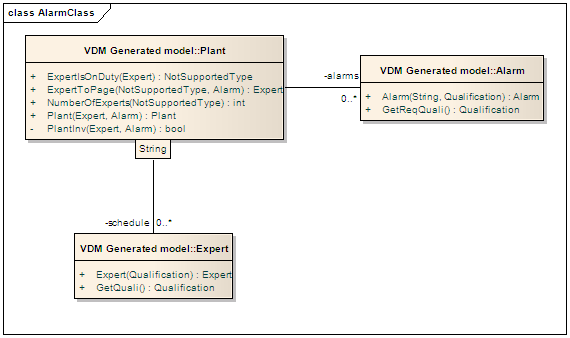
\includegraphics[width=5in]{figures/UMLFromVDM}
  \caption[labelInTOC]{UML diagram translated from VDM++ files}
  \label{fig:finalumlforalarm}
\end{center}
\end{figure}

%\begin{figure}[h]
%\begin{center}
%\includegraphics[width=3.5in]{seqdiagramforalarm}
%\caption{The Sequence Diagram for the traces inside the Alarm VDM++ model\label{fig:seqdiagforalarm}}
%\end{center}
%\end{figure}

\subsection{The Plant Class}

The \texttt{Plant} class is the main class in this example. 

\begin{lstlisting}
class Plant

instance variables

alarms   : set of Alarm;
schedule : map Period to set of Expert;
inv PlantInv(alarms,schedule);
\end{lstlisting}

\begin{lstlisting}
functions

PlantInv: set of Alarm * map Period to set of Expert -> 
          bool
PlantInv(as,sch) ==
  (forall p in set dom sch & sch(p) <> {}) and
  (forall a in set as &
     forall p in set dom sch &
       exists expert in set sch(p) &
         a.GetReqQuali() in set expert.GetQuali());

types

public Period = token;

operations

public ExpertToPage: Alarm * Period ==> Expert
ExpertToPage(a, p) ==
  let expert in set schedule(p) be st
      a.GetReqQuali() in set expert.GetQuali()
  in
    return expert
pre a in set alarms and
    p in set dom schedule
post let expert = RESULT
     in
       expert in set schedule(p) and
       a.GetReqQuali() in set expert.GetQuali();

public NumberOfExperts: Period ==> nat
NumberOfExperts(p) ==
  return card schedule(p)
pre p in set dom schedule;

public ExpertIsOnDuty: Expert ==> set of Period
ExpertIsOnDuty(ex) ==
  return {p | p in set dom schedule & 
              ex in set schedule(p)};

public Plant: set of Alarm * 
              map Period to set of Expert ==> Plant
Plant(als,sch) ==
( alarms := als;
  schedule := sch)
pre PlantInv(als,sch);

end Plant
\end{lstlisting}

\subsection{The Expert Class}

\begin{lstlisting}
class Expert

instance variables

quali : set of Qualification;

types
 
public Qualification = <Mech> | <Chem> | <Bio> | <Elec>;

operations

public Expert: set of Qualification ==> Expert
Expert(qs) ==
  quali := qs;

public GetQuali: () ==> set of Qualification
GetQuali() ==
  return quali;
  
end Expert
\end{lstlisting}

\subsection{the Alarm Class}

\begin{lstlisting}
class Alarm
types

public String = seq of char;

instance variables 

descr    : String;
reqQuali : Expert`Qualification;

operations

public Alarm: Expert`Qualification * String ==> Alarm
Alarm(quali,str) ==
( descr := str;
  reqQuali := quali
);
\end{lstlisting}

\begin{lstlisting}
public GetReqQuali: () ==> Expert`Qualification
GetReqQuali() ==
  return reqQuali;
  
end Alarm
\end{lstlisting}

\subsection{A Test Class}

\begin{lstlisting}
class Test1

instance variables

a1   : Alarm  := new Alarm(<Mech>,"Mechanical fault");
a2   : Alarm  := new Alarm(<Chem>,"Tank overflow");
ex1  : Expert := new Expert({<Mech>,<Bio>});
ex2  : Expert := new Expert({<Elec>});
ex3  : Expert := new Expert({<Chem>,<Bio>,<Mech>});
ex4  : Expert := new Expert({<Elec>,<Chem>});
plant: Plant  := new Plant({a1},{p1 |-> {ex1,ex4},
                                 p2 |-> {ex2,ex3}});

values

p1: Plant`Period = mk_token("Monday day");
p2: Plant`Period = mk_token("Monday night");
p3: Plant`Period = mk_token("Tuesday day");
p4: Plant`Period = mk_token("Tuesday night");

operations

public Run: () ==> set of Plant`Period * Expert
Run() == 
  let periods = plant.ExpertIsOnDuty(ex1),
      expert  = plant.ExpertToPage(a1,p1)
  in 
    return mk_(periods,expert);

end Test1
\end{lstlisting}



